\documentclass[10pt]{article}

% Article scientifique en colonne unique, compatible pdfLaTeX.
\usepackage[utf8]{inputenc}
\usepackage[T1]{fontenc}
\usepackage{natbib}
\usepackage[french,shorthands=off]{babel}
\usepackage{mathptmx}
\usepackage[left=1.0in,right=1.0in,top=0.9in,bottom=0.9in]{geometry}
\usepackage{microtype}
\usepackage{amsmath,amssymb}
\usepackage{graphicx}
\usepackage{booktabs}
\usepackage{tabularx}
\usepackage{array}
\usepackage{enumitem}
\usepackage{xcolor}
\usepackage{caption}
\usepackage[hidelinks]{hyperref}

\setlength{\parindent}{1em}
\setlength{\parskip}{0.25em}
\setlist{nosep,leftmargin=*}
\captionsetup{font=small,labelfont=bf}
\newcommand{\pgvector}{\texttt{pgvector}}
\newcommand{\neo}{\texttt{Neo4j}}
\newcommand{\langgraph}{\texttt{LangGraph}}
\newcommand{\ndcg}{\ensuremath{\mathrm{NDCG@10}}}
\newcommand{\mrr}{\ensuremath{\mathrm{MRR@10}}}
\newcommand{\recall}{\ensuremath{\mathrm{Recall@10}}}

\title{\textbf{Recherche sémantique et graphes de connaissances pour le matching emploi--compétences : conception et évaluation interne d'un pipeline hybride}}
\author{Irch Defluviaire NGOULOU NGOUBILI\\
\small Institut Sous-régional de Statistique et d'Économie Appliquée (ISSEA)\\
\small Option Data Science et Marketing\\
\small Encadrement : Dr FOUTSE Yuehgoh\\
\small Data Scientist, PhD Computer Science\\
\small \texttt{Mémoire professionnel -- version article scientifique}}
\date{Août 2026}

\begin{document}
\maketitle

\begin{abstract}
Le rapprochement entre profils de candidats et offres d'emploi reste difficile lorsque les compétences sont décrites avec des vocabulaires hétérogènes et que les systèmes de recommandation ne rendent pas leurs décisions explicites. Cet article présente un pipeline hybride de matching emploi--compétences combinant une recherche sémantique, un graphe de connaissances et une génération contrôlée. Le système harmonise 13\,957 offres, 41\,298 profils candidats et des référentiels métiers--compétences, puis adapte un encodeur SentenceTransformer avant d'indexer les représentations dans PostgreSQL/\pgvector{}. Les relations entre candidats, compétences, métiers, formations et offres sont modélisées dans \neo{} afin de calculer la couverture des compétences et le \textit{skill gap}. Sur 953 paires de test, l'encodeur adapté obtient une \ndcg{} de 0,6232, un \mrr{} de 0,5874 et un \recall{} de 0,7398. Dans une ablation contrôlée sur un même vivier initial de 30 offres, l'ajout du graphe fait progresser la \ndcg{} de 0,5575 à 0,7392 et le \mrr{} de 0,6908 à 0,8093 selon un proxy de pertinence. Ces résultats établissent une amélioration interne du classement et une capacité d'explication relationnelle, mais ne constituent pas encore une preuve d'utilité métier ou d'impact sur l'insertion professionnelle. L'article documente ainsi une architecture opérationnelle et les conditions nécessaires à sa validation externe.
\end{abstract}

\noindent\textbf{Mots-clés :} recherche sémantique ; systèmes de recommandation ; emploi--compétences ; embeddings ; graphe de connaissances ; GraphRAG ; skill gap.

\twocolumn

\section{Introduction}
L'appariement entre candidats et offres d'emploi est un problème de recommandation soumis à une forte hétérogénéité lexicale. Une même compétence peut être exprimée par un intitulé, une description d'expérience, un diplôme ou une formulation locale. Les approches par mots-clés sont alors sensibles à la surface textuelle, tandis que les systèmes fondés sur les interactions historiques exigent des données d'usage qui ne sont pas toujours disponibles dans les contextes émergents. Cette difficulté est également économique : l'information imparfaite et les frictions de recherche compliquent la rencontre entre l'offre et la demande de travail \citep{akerlof1970lemons,spence1973job,mortensen1994job,pissarides2000equilibrium}.

Les modèles de représentation dense permettent de comparer des textes selon leur proximité sémantique \citep{reimers2019sbert,muennighoff2022sgpt}. Cependant, une proximité vectorielle ne suffit pas toujours à expliquer la compatibilité professionnelle. Elle ne distingue pas nécessairement une compétence possédée d'une compétence requise, ne représente pas explicitement les chemins entre métiers et formations et peut reproduire les biais du corpus. Les graphes de connaissances fournissent une représentation complémentaire des entités et de leurs relations \citep{hogan2021knowledge,schlichtkrull2018rgcn}. Les systèmes de génération augmentée par récupération peuvent ensuite produire une réponse conditionnée par des preuves récupérées \citep{lewis2020rag}, sous réserve de contrôler la fidélité de la génération.

Cet article étudie donc la question suivante : \emph{dans quelle mesure la combinaison d'une recherche sémantique et d'un graphe de connaissances peut-elle améliorer le classement et l'explicabilité d'un système de matching emploi--compétences ?} Le travail apporte trois contributions :
\begin{itemize}
  \item un pipeline reproductible d'harmonisation, de représentation sémantique et de modélisation relationnelle pour des données d'emploi et de formation ;
  \item un moteur hybride qui utilise \pgvector{} pour constituer un vivier puis \neo{} pour calculer la couverture et le \textit{skill gap} ;
  \item une évaluation interne séparant le benchmark de l'encodeur, l'ablation du graphe, le réglage des poids et le contrôle de génération.
\end{itemize}
Les conclusions sont volontairement limitées à la faisabilité et aux performances internes mesurées avec les données disponibles. La pertinence métier n'est pas assimilée au proxy utilisé pour l'évaluation.

\section{Travaux connexes}
Les systèmes de recommandation fondés sur le contenu comparent les attributs des objets et du profil, alors que les approches collaboratives exploitent les historiques d'interactions \citep{pazzani2007content,koren2009matrix,ricci2011recommender}. Dans le recrutement, ces historiques sont souvent incomplets et les interactions observées peuvent refléter des pratiques de sélection plutôt que la compétence réelle. Les modèles hybrides cherchent à combiner plusieurs signaux afin de réduire cette dépendance à une seule représentation \citep{burke2002hybrid}.

Les encodeurs de phrases transforment un texte en vecteur dense utilisable pour le retrieval. Sentence-BERT a popularisé l'apprentissage de représentations adaptées à la comparaison de phrases \citep{reimers2019sbert}; les travaux de recherche sémantique évaluent notamment le rang du premier résultat et la qualité du top-$k$ \citep{thakur2021beir,muennighoff2022mteb}. Dans le domaine des compétences, les graphes peuvent représenter les relations entre métiers, compétences et offres, et les méthodes neuronales peuvent exploiter leur structure \citep{goyal2023jobxmlc,he2020lightgcn}.

La génération augmentée par récupération réduit la dépendance aux connaissances paramétriques du modèle en lui fournissant un contexte externe \citep{lewis2020rag}. Les variantes GraphRAG ajoutent une navigation relationnelle, mais elles ne rendent pas automatiquement les données vraies : une réponse peut être fidèle à un contexte incomplet. Les workflows agentiques ajoutent une planification, des outils et une boucle de vérification \citep{yao2023react,asai2024selfrag}. Le présent travail se situe à l'intersection de ces approches, avec une architecture orientée vers l'explication du matching plutôt que vers la seule génération de texte.

\section{Méthodologie}
\subsection{Données et normalisation}
Le corpus exploité contient 13\,957 offres et 41\,298 profils candidats. Il est complété par des référentiels de compétences et de professions, notamment ESCO \citep{europeancommission2024esco}, ainsi que par des nomenclatures camerounaises des métiers et des formations \citep{minfop2013ncm}. Les données sont extraites, nettoyées et transformées dans une chaîne ETL. Les champs bruts sont conservés pour la traçabilité ; des champs normalisés décrivent le titre, le secteur, la localisation, le contrat, l'expérience, le niveau de qualification et les compétences.

\begin{table}[ht]
\centering
\caption{Composition synthétique du corpus exploité}
\label{tab:data}
\small
\begin{tabularx}{\linewidth}{>{\raggedright\arraybackslash}X r >{\raggedright\arraybackslash}X}
\toprule
Composante & Effectif & Fonction dans le pipeline \\
\midrule
Offres d'emploi & 13\,957 & Retrieval et recommandations \\
Profils candidats & 41\,298 & Requêtes et calcul du skill gap \\
Compétences ESCO & 13\,939 & Normalisation et relations \\
Professions ESCO & 3\,039 & Enrichissement métier \\
Paires offre--description & 6\,476 & Fine-tuning de l'encodeur \\
\bottomrule
\end{tabularx}
\end{table}

Les textes destinés à l'encodage combinent les informations structurées et les descriptions nettoyées. Les diplômes et formations sont alignés sur des niveaux de qualification afin de limiter les divergences de codage. Les relations métiers--compétences issues des référentiels servent à enrichir le graphe et à distinguer la compétence directement déclarée de la compétence associée à un métier.

La chaîne complète est organisée selon une séparation entre préparation, récupération, vérification et génération. Cette séparation permet d'identifier la contribution de chaque brique et limite le risque qu'un modèle génératif produise une recommandation sans preuve exploitable.

\begin{figure}[ht]
\centering
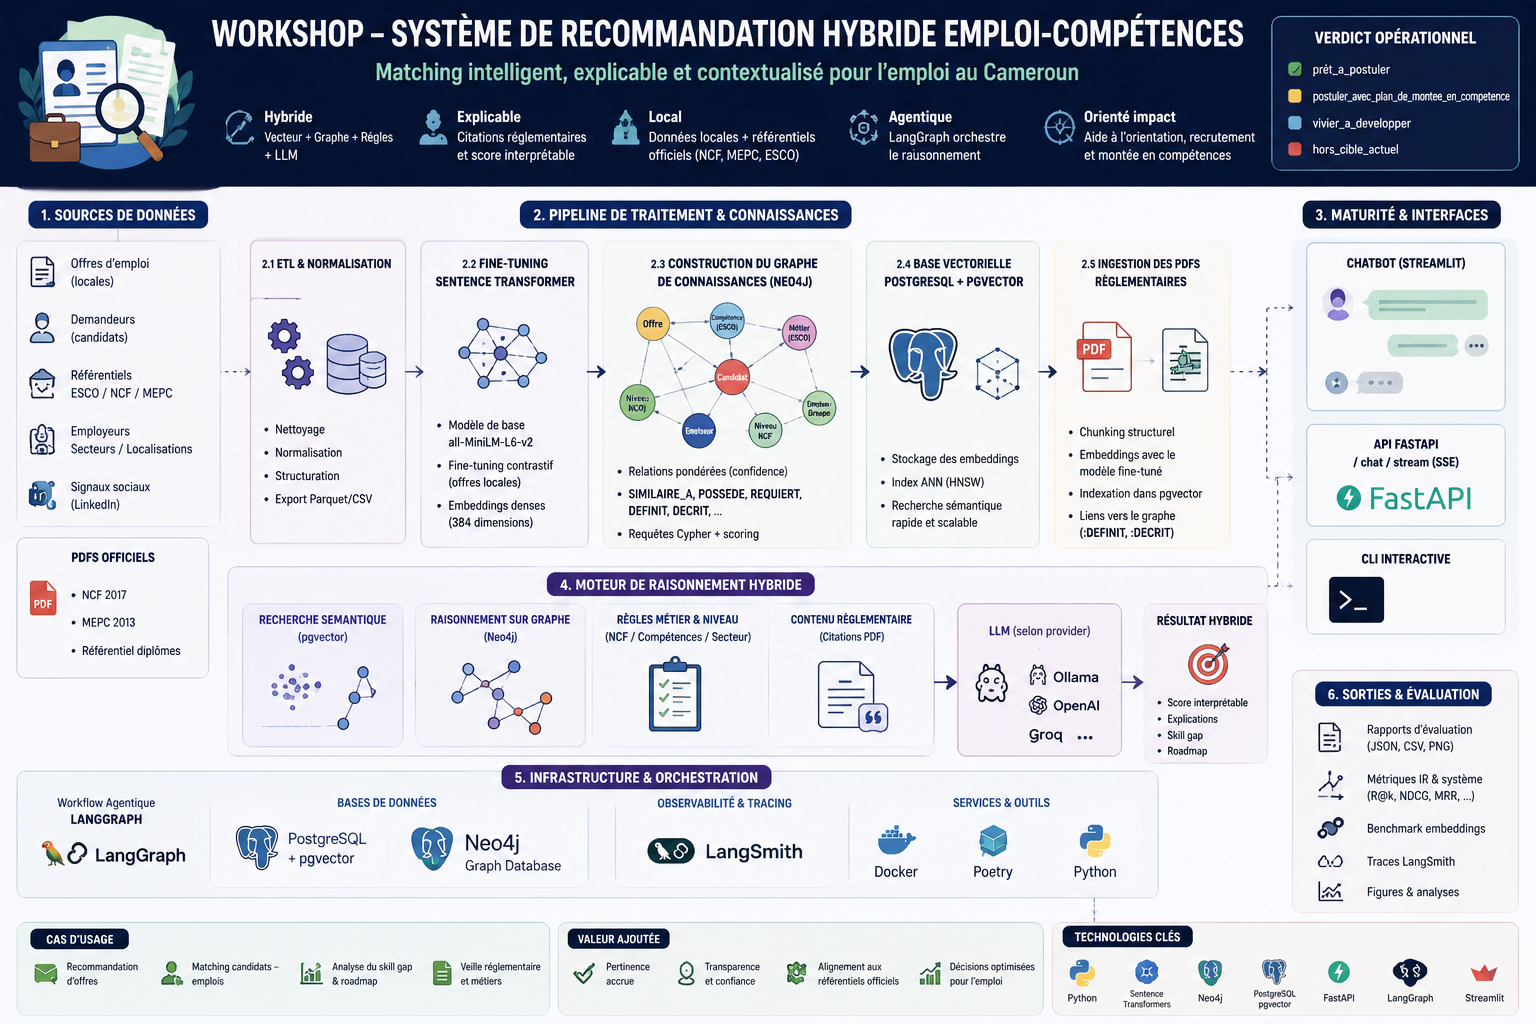
\includegraphics[width=0.96\linewidth]{figures/approche.png}
\caption{Vue synthétique du pipeline hybride : normalisation, représentation vectorielle, graphe relationnel et génération contrôlée.}
\label{fig:pipeline}
\end{figure}

\subsection{Représentation sémantique et fine-tuning}
Le modèle de base est \texttt{all-MiniLM-L6-v2}, un encodeur dense produisant des vecteurs de 384 dimensions. Le fine-tuning utilise 6\,476 paires offre--description, réparties en 4\,542 observations d'entraînement, 981 de validation et 953 de test. L'apprentissage est réalisé pendant cinq époques, avec une taille de lot de 32, un taux maximal de $2\times10^{-5}$ et une \textit{Multiple Negatives Ranking Loss}. Les autres descriptions du lot jouent le rôle de négatifs implicites.

Pour une requête $q$ et une offre $o$, la recherche vectorielle utilise une similarité cosinus :
\begin{equation}
 s_{\mathrm{vec}}(q,o)=\frac{e(q)\cdot e(o)}{\lVert e(q)\rVert_2\lVert e(o)\rVert_2}.
\end{equation}
Les vecteurs sont stockés et interrogés dans PostgreSQL avec l'index \pgvector{}. Cette étape constitue un vivier initial d'offres sémantiquement proches ; elle ne fournit pas, à elle seule, une explication relationnelle.

\subsection{Graphe et moteur hybride}
Le graphe contient notamment des nœuds \texttt{Candidat}, \texttt{Offre}, \texttt{Compétence}, \texttt{Métier} et \texttt{Formation}. Le chemin central est représenté par
\[
\texttt{Candidat-POSSEDE-Compétence-REQUIERT-Offre}.
\]
Pour un couple candidat--offre, la couverture des compétences est définie par :
\begin{equation}
 s_{\mathrm{graph}}(c,o)=\frac{|K_c\cap K_o|}{|K_o|},
\end{equation}
où $K_c$ désigne les compétences du candidat et $K_o$ les compétences requises par l'offre. Le \textit{skill gap} est $K_o\setminus K_c$, avec une attention particulière aux compétences nécessaires au métier et au niveau de qualification.

Le moteur hybride reclasse le vivier selon :
\begin{equation}
 s_{\mathrm{hyb}}(c,o)=\alpha s_{\mathrm{vec}}(c,o)+\beta s_{\mathrm{graph}}(c,o),\qquad \alpha+\beta=1.
\end{equation}
Les poids sont calibrés sur 690 couples associés à 69 candidats évalués. Cette calibration ne doit pas être interprétée comme une preuve qu'un poids est universel : elle dépend du proxy, du vivier présélectionné et de la fonction objectif.

\subsection{Orchestration et génération contrôlée}
Le workflow \langgraph{} analyse l'intention, sélectionne les outils, exécute les requêtes, construit un contexte et transmet les preuves au LLM final. Une recommandation mobilise \pgvector{} et \neo{} ; une question sur les référentiels mobilise la recherche documentaire ; une question relationnelle peut utiliser Text-to-Cypher, sous contrôle du schéma. Un critic compare ensuite la réponse aux éléments du contexte et renvoie une décision \texttt{accept} ou \texttt{revise}. Le seuil calibré est de 0,46 sur un test contrastif de 102 comparaisons.

\subsection{Protocole d'évaluation}
Le benchmark de représentation évalue le modèle sur les 953 paires de test avec la \ndcg{}, le \mrr{} et le \recall{}. L'ablation compare deux variantes sur le même pool de 30 offres par candidat : \texttt{pgvector seul} conserve l'ordre vectoriel ; \texttt{pgvector + graphe} reclasse le même pool avec la couverture relationnelle. Le proxy de pertinence combine recouvrement lexical, compatibilité sectorielle et niveau de qualification. Il sert de référence commune, mais ne remplace pas une annotation humaine.

\section{Résultats}
\subsection{Benchmark de l'encodeur}
Le modèle adapté obtient une \ndcg{} de 0,6232, un \mrr{} de 0,5874 et un \recall{} de 0,7398 sur les données de test. Ces métriques montrent que le fine-tuning améliore la récupération des descriptions associées dans la tâche construite. Elles ne mesurent cependant ni la satisfaction d'un recruteur ni la qualité d'une embauche.

\begin{table}[ht]
\centering
\caption{Performance du modèle adapté sur les 953 paires de test}
\label{tab:embedding}
\small
\begin{tabularx}{\linewidth}{>{\raggedright\arraybackslash}X c c c}
\toprule
Modèle & \ndcg{} & \mrr{} & \recall{} \\
\midrule
SentenceTransformer adapté & 0,6232 & 0,5874 & 0,7398 \\
\bottomrule
\end{tabularx}
\end{table}

\subsection{Ablation du graphe}
Le tableau~\ref{tab:ablation} compare les deux variantes sur le même vivier. Le graphe augmente la \ndcg{} de 0,1817, le \mrr{} de 0,1185 et le \recall{} de 0,1656. L'amélioration est cohérente avec la fonction du graphe : il apporte un signal de couverture et des explications de compétences, tandis que la recherche vectorielle assure le rappel initial.

\begin{table}[ht]
\centering
\caption{Ablation sur le même pool initial, selon le proxy de pertinence}
\label{tab:ablation}
\small
\begin{tabularx}{\linewidth}{>{\raggedright\arraybackslash}X c c c}
\toprule
Variante & \ndcg{} & \mrr{} & \recall{} \\
\midrule
\pgvector{} seul & 0,5575 & 0,6908 & 0,4491 \\
\pgvector{} + graphe & 0,7392 & 0,8093 & 0,6147 \\
\bottomrule
\end{tabularx}
\end{table}

La comparaison est informative parce que le pool initial est maintenu constant. Elle reste néanmoins une évaluation par proxy. Le gain ne peut donc pas être formulé comme une amélioration de la pertinence réelle des recrutements. En outre, 11 des 80 candidats tirés initialement n'ont pas pu être évalués en raison d'erreurs techniques ; les résultats portent sur 69 candidats.

\subsection{Calibration et critic}
Après 500 essais Optuna \citep{akiba2019optuna}, l'objectif fondé sur la \ndcg{} retient la frontière \texttt{Neo4j seul} dans le vivier déjà présélectionné par \pgvector{}, avec une valeur de 0,9697 selon le proxy. Pour l'objectif combinant \mrr{} et précision, le compromis est de 0,6615 pour le signal vectoriel et de 0,3385 pour le signal relationnel. Cette différence montre qu'il n'existe pas de poids optimal indépendant de la fonction objectif et de l'échantillon.

Le critic accepte 50 des 51 contextes réels et rejette les 51 contextes mélangés au seuil 0,46. Ce test documente une capacité de contrôle lexical dans le protocole utilisé. Il ne garantit pas la vérité métier, la complétude du contexte ou l'absence d'hallucination dans des situations non testées.

\section{Discussion et limites}
Les résultats soutiennent l'intérêt d'une architecture en deux mémoires. \pgvector{} fournit une représentation continue et un rappel sémantique ; \neo{} encode des relations explicites, calcule la couverture et expose le \textit{skill gap}. L'intérêt principal du pipeline n'est donc pas seulement l'amélioration d'une métrique, mais la séparation fonctionnelle entre recherche, vérification et explication.

Trois limites réduisent cependant la portée des conclusions. Premièrement, le proxy de pertinence est construit à partir de signaux disponibles dans les données et peut favoriser les critères qu'il réutilise. Deuxièmement, l'absence d'annotations indépendantes de recruteurs empêche d'estimer une pertinence métier de référence. Troisièmement, l'échantillon d'ablation est limité et comporte des échecs techniques ; aucune validation utilisateur ne mesure encore la compréhension ou l'utilité des explications.

Le corpus peut également contenir des biais de couverture, de secteur, de localisation et de collecte. Les résultats ne permettent donc pas d'affirmer une généralisation à l'ensemble du marché camerounais, encore moins une amélioration causale de l'emploi. Une validation future devrait inclure un jeu annoté par plusieurs recruteurs, une mesure de l'accord inter-évaluateurs, des tests utilisateurs, une analyse par sous-groupes et une évaluation temporelle hors échantillon. La reproductibilité exige en outre la publication des scripts, des versions de données, des paramètres d'indexation et des journaux d'exécution, sous réserve des contraintes de confidentialité.

\section{Conclusion}
Cet article a présenté un pipeline hybride pour le matching emploi--compétences combinant embeddings, recherche vectorielle, graphe de connaissances et génération contrôlée. Le modèle adapté obtient de bonnes performances dans le benchmark construit, et l'ablation indique un gain du graphe sur le même vivier initial selon le proxy disponible. Le système fournit en outre une représentation explicite des compétences couvertes et manquantes.

La conclusion défendable est celle d'une faisabilité technique et d'un apport interne mesurable du graphe, non celle d'une preuve d'impact sur le recrutement. La prochaine étape scientifique consiste à remplacer le proxy par des annotations humaines, à évaluer l'utilité des explications et à étudier la robustesse du système selon les secteurs, les niveaux de qualification et les sources de données.

\section*{Déclaration sur l'utilisation d'outils d'IA}
Les outils d'intelligence artificielle peuvent avoir été utilisés comme assistants de rédaction, de reformulation ou de programmation. Les auteurs restent responsables de la vérification des données, des méthodes, des résultats, des références et de la version finale du manuscrit. La déclaration définitive doit être adaptée aux règles de la revue ou de la conférence ciblée.

\bibliographystyle{unsrtnat}
\bibliography{references}

\end{document}
